\item Se a um cilindro $A$ é dada uma velocidade descendente inicial de \SI{2}{\meter/\second}, determine a velocidade de cada cilindro quando $t=\SI{3}{\second}$. Despreze a massa das polias.

\import{sections/answers/}{answer-7}

\vspace{-1.8cm}
\begin{flushright}
	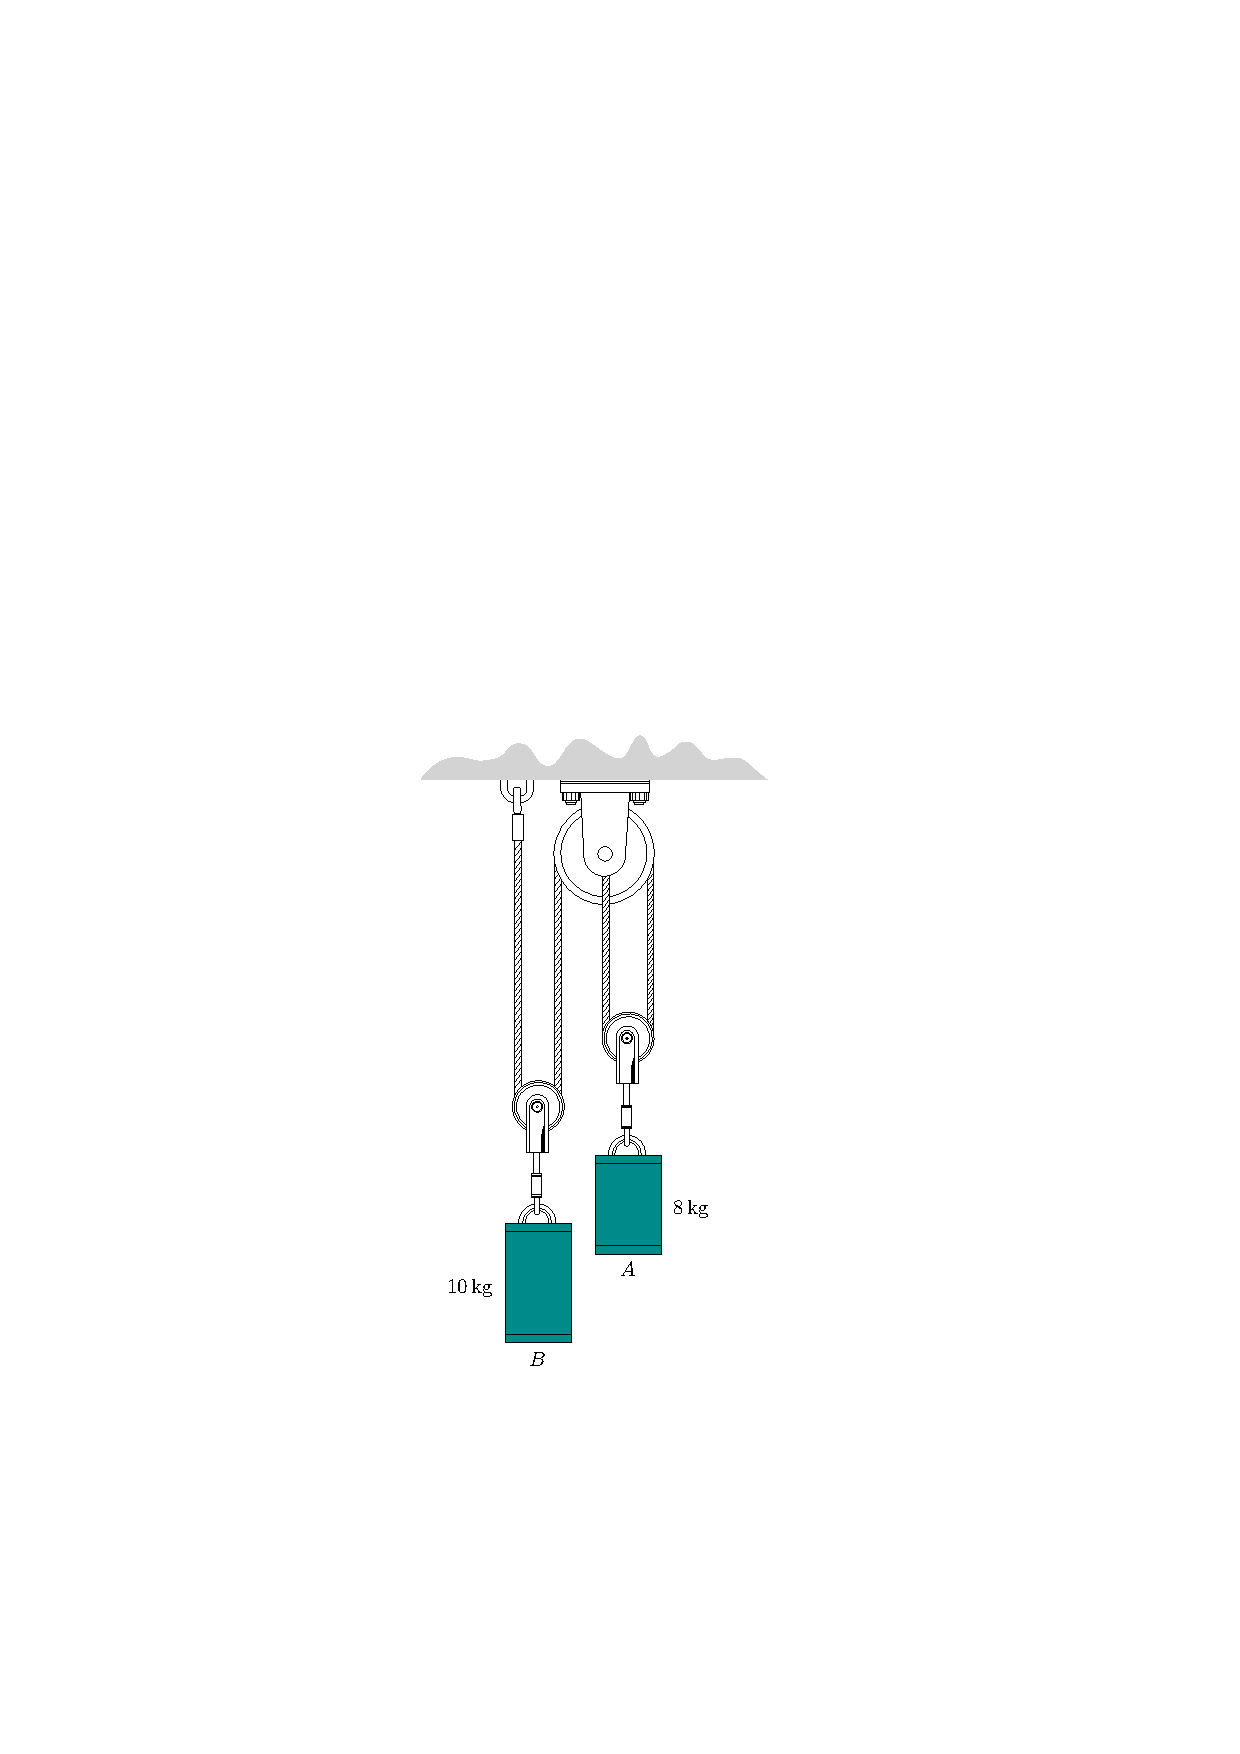
\includegraphics[scale=1.3]{images/draw_7}
\end{flushright}